
%% bare_conf.tex
%% V1.4
%% 2012/12/27
%% by Michael Shell
%% See:
%% http://www.michaelshell.org/
%% for current contact information.
%%
%% This is a skeleton file demonstrating the use of IEEEtran.cls
%% (requires IEEEtran.cls version 1.8 or later) with an IEEE conference paper.
%%
%% Support sites:
%% http://www.michaelshell.org/tex/ieeetran/
%% http://www.ctan.org/tex-archive/macros/latex/contrib/IEEEtran/
%% and
%% http://www.ieee.org/

%%*************************************************************************
%% Legal Notice:
%% This code is offered as-is without any warranty either expressed or
%% implied; without even the implied warranty of MERCHANTABILITY or
%% FITNESS FOR A PARTICULAR PURPOSE! 
%% User assumes all risk.
%% In no event shall IEEE or any contributor to this code be liable for
%% any damages or losses, including, but not limited to, incidental,
%% consequential, or any other damages, resulting from the use or misuse
%% of any information contained here.
%%
%% All comments are the opinions of their respective authors and are not
%% necessarily endorsed by the IEEE.
%%
%% This work is distributed under the LaTeX Project Public License (LPPL)
%% ( http://www.latex-project.org/ ) version 1.3, and may be freely used,
%% distributed and modified. A copy of the LPPL, version 1.3, is included
%% in the base LaTeX documentation of all distributions of LaTeX released
%% 2003/12/01 or later.
%% Retain all contribution notices and credits.
%% ** Modified files should be clearly indicated as such, including  **
%% ** renaming them and changing author support contact information. **
%%
%% File list of work: IEEEtran.cls, IEEEtran_HOWTO.pdf, bare_adv.tex,
%%                    bare_conf.tex, bare_jrnl.tex, bare_jrnl_compsoc.tex,
%%                    bare_jrnl_transmag.tex
%%*************************************************************************

% *** Authors should verify (and, if needed, correct) their LaTeX system  ***
% *** with the testflow diagnostic prior to trusting their LaTeX platform ***
% *** with production work. IEEE's font choices can trigger bugs that do  ***
% *** not appear when using other class files.                            ***
% The testflow support page is at:
% http://www.michaelshell.org/tex/testflow/



% Note that the a4paper option is mainly intended so that authors in
% countries using A4 can easily print to A4 and see how their papers will
% look in print - the typesetting of the document will not typically be
% affected with changes in paper size (but the bottom and side margins will).
% Use the testflow package mentioned above to verify correct handling of
% both paper sizes by the user's LaTeX system.
%
% Also note that the "draftcls" or "draftclsnofoot", not "draft", option
% should be used if it is desired that the figures are to be displayed in
% draft mode.
%
\documentclass[conference]{IEEEtran}
% Add the compsoc option for Computer Society conferences.
%
% If IEEEtran.cls has not been installed into the LaTeX system files,
% manually specify the path to it like:
% \documentclass[conference]{../sty/IEEEtran}





% Some very useful LaTeX packages include:
% (uncomment the ones you want to load)


% *** MISC UTILITY PACKAGES ***
%
%\usepackage{ifpdf}
% Heiko Oberdiek's ifpdf.sty is very useful if you need conditional
% compilation based on whether the output is pdf or dvi.
% usage:
% \ifpdf
%   % pdf code
% \else
%   % dvi code
% \fi
% The latest version of ifpdf.sty can be obtained from:
% http://www.ctan.org/tex-archive/macros/latex/contrib/oberdiek/
% Also, note that IEEEtran.cls V1.7 and later provides a builtin
% \ifCLASSINFOpdf conditional that works the same way.
% When switching from latex to pdflatex and vice-versa, the compiler may
% have to be run twice to clear warning/error messages.






% *** CITATION PACKAGES ***
%
%\usepackage{cite}
% cite.sty was written by Donald Arseneau
% V1.6 and later of IEEEtran pre-defines the format of the cite.sty package
% \cite{} output to follow that of IEEE. Loading the cite package will
% result in citation numbers being automatically sorted and properly
% "compressed/ranged". e.g., [1], [9], [2], [7], [5], [6] without using
% cite.sty will become [1], [2], [5]--[7], [9] using cite.sty. cite.sty's
% \cite will automatically add leading space, if needed. Use cite.sty's
% noadjust option (cite.sty V3.8 and later) if you want to turn this off
% such as if a citation ever needs to be enclosed in parenthesis.
% cite.sty is already installed on most LaTeX systems. Be sure and use
% version 4.0 (2003-05-27) and later if using hyperref.sty. cite.sty does
% not currently provide for hyperlinked citations.
% The latest version can be obtained at:
% http://www.ctan.org/tex-archive/macros/latex/contrib/cite/
% The documentation is contained in the cite.sty file itself.






% *** GRAPHICS RELATED PACKAGES ***
%
\ifCLASSINFOpdf
  % \usepackage[pdftex]{graphicx}
  % declare the path(s) where your graphic files are
  % \graphicspath{{../pdf/}{../jpeg/}}
  % and their extensions so you won't have to specify these with
  % every instance of \includegraphics
  % \DeclareGraphicsExtensions{.pdf,.jpeg,.png}
\else
  % or other class option (dvipsone, dvipdf, if not using dvips). graphicx
  % will default to the driver specified in the system graphics.cfg if no
  % driver is specified.
  % \usepackage[dvips]{graphicx}
  % declare the path(s) where your graphic files are
  % \graphicspath{{../eps/}}
  % and their extensions so you won't have to specify these with
  % every instance of \includegraphics
  % \DeclareGraphicsExtensions{.eps}
\fi
% graphicx was written by David Carlisle and Sebastian Rahtz. It is
% required if you want graphics, photos, etc. graphicx.sty is already
% installed on most LaTeX systems. The latest version and documentation
% can be obtained at: 
% http://www.ctan.org/tex-archive/macros/latex/required/graphics/
% Another good source of documentation is "Using Imported Graphics in
% LaTeX2e" by Keith Reckdahl which can be found at:
% http://www.ctan.org/tex-archive/info/epslatex/
%
% latex, and pdflatex in dvi mode, support graphics in encapsulated
% postscript (.eps) format. pdflatex in pdf mode supports graphics
% in .pdf, .jpeg, .png and .mps (metapost) formats. Users should ensure
% that all non-photo figures use a vector format (.eps, .pdf, .mps) and
% not a bitmapped formats (.jpeg, .png). IEEE frowns on bitmapped formats
% which can result in "jaggedy"/blurry rendering of lines and letters as
% well as large increases in file sizes.
%
% You can find documentation about the pdfTeX application at:
% http://www.tug.org/applications/pdftex





% *** MATH PACKAGES ***
%
%\usepackage[cmex10]{amsmath}
% A popular package from the American Mathematical Society that provides
% many useful and powerful commands for dealing with mathematics. If using
% it, be sure to load this package with the cmex10 option to ensure that
% only type 1 fonts will utilized at all point sizes. Without this option,
% it is possible that some math symbols, particularly those within
% footnotes, will be rendered in bitmap form which will result in a
% document that can not be IEEE Xplore compliant!
%
% Also, note that the amsmath package sets \interdisplaylinepenalty to 10000
% thus preventing page breaks from occurring within multiline equations. Use:
%\interdisplaylinepenalty=2500
% after loading amsmath to restore such page breaks as IEEEtran.cls normally
% does. amsmath.sty is already installed on most LaTeX systems. The latest
% version and documentation can be obtained at:
% http://www.ctan.org/tex-archive/macros/latex/required/amslatex/math/





% *** SPECIALIZED LIST PACKAGES ***
%
%\usepackage{algorithmic}
% algorithmic.sty was written by Peter Williams and Rogerio Brito.
% This package provides an algorithmic environment fo describing algorithms.
% You can use the algorithmic environment in-text or within a figure
% environment to provide for a floating algorithm. Do NOT use the algorithm
% floating environment provided by algorithm.sty (by the same authors) or
% algorithm2e.sty (by Christophe Fiorio) as IEEE does not use dedicated
% algorithm float types and packages that provide these will not provide
% correct IEEE style captions. The latest version and documentation of
% algorithmic.sty can be obtained at:
% http://www.ctan.org/tex-archive/macros/latex/contrib/algorithms/
% There is also a support site at:
% http://algorithms.berlios.de/index.html
% Also of interest may be the (relatively newer and more customizable)
% algorithmicx.sty package by Szasz Janos:
% http://www.ctan.org/tex-archive/macros/latex/contrib/algorithmicx/




% *** ALIGNMENT PACKAGES ***
%
%\usepackage{array}
% Frank Mittelbach's and David Carlisle's array.sty patches and improves
% the standard LaTeX2e array and tabular environments to provide better
% appearance and additional user controls. As the default LaTeX2e table
% generation code is lacking to the point of almost being broken with
% respect to the quality of the end results, all users are strongly
% advised to use an enhanced (at the very least that provided by array.sty)
% set of table tools. array.sty is already installed on most systems. The
% latest version and documentation can be obtained at:
% http://www.ctan.org/tex-archive/macros/latex/required/tools/


% IEEEtran contains the IEEEeqnarray family of commands that can be used to
% generate multiline equations as well as matrices, tables, etc., of high
% quality.




% *** SUBFIGURE PACKAGES ***
%\ifCLASSOPTIONcompsoc
%  \usepackage[caption=false,font=normalsize,labelfont=sf,textfont=sf]{subfig}
%\else
%  \usepackage[caption=false,font=footnotesize]{subfig}
%\fi
% subfig.sty, written by Steven Douglas Cochran, is the modern replacement
% for subfigure.sty, the latter of which is no longer maintained and is
% incompatible with some LaTeX packages including fixltx2e. However,
% subfig.sty requires and automatically loads Axel Sommerfeldt's caption.sty
% which will override IEEEtran.cls' handling of captions and this will result
% in non-IEEE style figure/table captions. To prevent this problem, be sure
% and invoke subfig.sty's "caption=false" package option (available since
% subfig.sty version 1.3, 2005/06/28) as this is will preserve IEEEtran.cls
% handling of captions.
% Note that the Computer Society format requires a larger sans serif font
% than the serif footnote size font used in traditional IEEE formatting
% and thus the need to invoke different subfig.sty package options depending
% on whether compsoc mode has been enabled.
%
% The latest version and documentation of subfig.sty can be obtained at:
% http://www.ctan.org/tex-archive/macros/latex/contrib/subfig/




% *** FLOAT PACKAGES ***
%
%\usepackage{fixltx2e}
% fixltx2e, the successor to the earlier fix2col.sty, was written by
% Frank Mittelbach and David Carlisle. This package corrects a few problems
% in the LaTeX2e kernel, the most notable of which is that in current
% LaTeX2e releases, the ordering of single and double column floats is not
% guaranteed to be preserved. Thus, an unpatched LaTeX2e can allow a
% single column figure to be placed prior to an earlier double column
% figure. The latest version and documentation can be found at:
% http://www.ctan.org/tex-archive/macros/latex/base/


%\usepackage{stfloats}
% stfloats.sty was written by Sigitas Tolusis. This package gives LaTeX2e
% the ability to do double column floats at the bottom of the page as well
% as the top. (e.g., "\begin{figure*}[!b]" is not normally possible in
% LaTeX2e). It also provides a command:
%\fnbelowfloat
% to enable the placement of footnotes below bottom floats (the standard
% LaTeX2e kernel puts them above bottom floats). This is an invasive package
% which rewrites many portions of the LaTeX2e float routines. It may not work
% with other packages that modify the LaTeX2e float routines. The latest
% version and documentation can be obtained at:
% http://www.ctan.org/tex-archive/macros/latex/contrib/sttools/
% Do not use the stfloats baselinefloat ability as IEEE does not allow
% \baselineskip to stretch. Authors submitting work to the IEEE should note
% that IEEE rarely uses double column equations and that authors should try
% to avoid such use. Do not be tempted to use the cuted.sty or midfloat.sty
% packages (also by Sigitas Tolusis) as IEEE does not format its papers in
% such ways.
% Do not attempt to use stfloats with fixltx2e as they are incompatible.
% Instead, use Morten Hogholm'a dblfloatfix which combines the features
% of both fixltx2e and stfloats:
%
% \usepackage{dblfloatfix}
% The latest version can be found at:
% http://www.ctan.org/tex-archive/macros/latex/contrib/dblfloatfix/




% *** PDF, URL AND HYPERLINK PACKAGES ***
%
%\usepackage{url}
% url.sty was written by Donald Arseneau. It provides better support for
% handling and breaking URLs. url.sty is already installed on most LaTeX
% systems. The latest version and documentation can be obtained at:
% http://www.ctan.org/tex-archive/macros/latex/contrib/url/
% Basically, \url{my_url_here}.




% *** Do not adjust lengths that control margins, column widths, etc. ***
% *** Do not use packages that alter fonts (such as pslatex).         ***
% There should be no need to do such things with IEEEtran.cls V1.6 and later.
% (Unless specifically asked to do so by the journal or conference you plan
% to submit to, of course. )
\usepackage{graphicx}
\usepackage{float}
%\usepackage{subfigure}
\usepackage{caption}
\usepackage{subcaption}
\usepackage{array}
\usepackage{amsmath}
\newcolumntype{C}[1]{>{\centering\let\newline\\\arraybackslash\hspace{0pt}}m{#1}}
\newcolumntype{L}[1]{>{\raggedright\let\newline\\\arraybackslash\hspace{0pt}}m{#1}}
%\usepackage{cite}
\usepackage[utf8]{inputenc}
\usepackage[english]{babel}
\usepackage{fancyhdr}
\usepackage{lastpage}
\usepackage{multirow}
 
\pagestyle{fancy}
\fancyhf{}
 
\rfoot{Page \thepage \hspace{1pt} of \pageref{LastPage}}
% correct bad hyphenation here
\hyphenation{op-tical net-works semi-conduc-tor}


\begin{document}
%
% paper title
% can use linebreaks \\ within to get better formatting as desired
% Do not put math or special symbols in the title.
\title{Canny Edge Detection Algorithm Implementation on Beagleboard}


% author names and affiliations
% use a multiple column layout for up to three different
% affiliations
\author{\IEEEauthorblockN{Andri Ramadhani, Angga Irawan, Arif Nurhidayat, Bontor Humala, Pengqi Chen, Rizky Dharmawan}
        
\IEEEauthorblockA{Embedded System Laboratory Assignment 2 Group 01\\
Delft University of Technology, Netherlands\\
Email: a.rahmadhani@student.tudelft.nl (4505611), anggairawan@student.tudelft.nl (4516974),\\
a.nurhidayat@student.tudelft.nl (4467388),
bontorhumala@student.tudelft.nl (4518993),\\ p.chen-1@student.tudelft.nl (4522354), rizkydharmawan@student.tudelft.nl (4501225) }
%\and
%\IEEEauthorblockN{Homer Simpson}
%\IEEEauthorblockA{Twentieth Century Fox\\
%Springfield, USA\\
%Email: homer@thesimpsons.com}
%\and
%\IEEEauthorblockN{James Kirk\\ and Montgomery Scott}
%\IEEEauthorblockA{Starfleet Academy\\
%San Francisco, California 96678-2391\\
%Telephone: (800) 555--1212\\
%Fax: (888) 555--1212}}
% conference papers do not typically use \thanks and this command
% is locked out in conference mode. If really needed, such as for
% the acknowledgment of grants, issue a \IEEEoverridecommandlockouts
% after \documentclass

% for over three affiliations, or if they all won't fit within the width
% of the page, use this alternative format:
% 
%\author{\IEEEauthorblockN{Michael Shell\IEEEauthorrefmark{1},
%Homer Simpson\IEEEauthorrefmark{2},
%James Kirk\IEEEauthorrefmark{3}, 
%Montgomery Scott\IEEEauthorrefmark{3} and
%Eldon Tyrell\IEEEauthorrefmark{4}}
%\IEEEauthorblockA{\IEEEauthorrefmark{1}School of Electrical and Computer Engineering\\
%Georgia Institute of Technology,
%Atlanta, Georgia 30332--0250\\ Email: see http://www.michaelshell.org/contact.html}
%\IEEEauthorblockA{\IEEEauthorrefmark{2}Twentieth Century Fox, Springfield, USA\\
%Email: homer@thesimpsons.com}
%\IEEEauthorblockA{\IEEEauthorrefmark{3}Starfleet Academy, San Francisco, California 96678-2391\\
%Telephone: (800) 555--1212, Fax: (888) 555--1212}
%\IEEEauthorblockA{\IEEEauthorrefmark{4}Tyrell Inc., 123 Replicant Street, Los Angeles, California 90210--4321}
}




% use for special paper notices
%\IEEEspecialpapernotice{(Invited Paper)}




% make the title area
\maketitle

% in the abstract
\begin{abstract}
Canny Edge Detection is a well-known edge detection algorithm, which has been proven to provide superior result compared to other methods. However, it also has slower execution time due to its heavy computation on floating point and intense matrix operation. Profiling the baseline program shows that around 78\% of the processing time is spent in the gaussian-smooth function. In this paper, implementation of canny edge detection algorithm on Beagleboard platform which has NEON feature in its General Purposed Processing unit (GPP) and a dedicated Digital Signal Processor (DSP) is discussed. The result shows that by converting floating point operation into fixed point operation, and load balancing gaussian-smooth function, i.e., performing the computation parallely 38\% in GPP using NEON with and 62 \%in DSP, a speed up factor of 2.1 compared to the baseline program was achieved.

\end{abstract}

\begin{IEEEkeywords}
Beagleboard, Canny edge detection, DSP, NEON, load balancing.
\end{IEEEkeywords}

\IEEEpeerreviewmaketitle


\section{Introduction}
Edge detection is an important step in image processing algorithm, and among many edge detector algorithms, canny edge detector is the most commonly used algorithm for many years due to its superior performance \cite{paper1}. However, due to its complex computation that involves floating point and matrices operations especially in the gaussian smooth procedure, it has considerably long computation time.

In this paper, the result of canny edge detection algorithm, which was applied on the Beagleboard\footnote{http://beagleboard.org/}, is discussed. Our target is to enhance the computation performance so that it runs as twice faster compared to the baseline without any algorithm modification. The Beagleboard has a general purpose ARM processor (GPP) that features NEON, which can perfom vector multiplication, and a dedicated digital signal processor (DSP), which can perform the computation in parallel with the GPP. In addition, floating point operation, which was done in both DSP and GPP, was also converted to fixed point operation to again enhance the computation speed. At the end, the Execution time and the picture generated by the modified and baseline canny edge program were compared and analyzed.

The rest of the paper is organized as follows. Section 2 addresses the problem to be solved and also the solution hypothesis. Section 3 presents the implementation of the canny edge algortihm on the Beagleboard, includes the optimizations performed in the solution hypothesis to speed up the execution time. The analysis and quantitative comparison of the execution time and the picture generated by the modified and baseline canny edge algorithm is presented in Section 4. Finally, the conclusion of the experiment is explained in Section 5.

\section{Problem statement}
% Here we define the problem statement as mentioned in the slide, and in addition the requirement proposed by the TA:
% – Profiling and	analysis of the algorithm
% – The execution on ARM/DSP/FPGA	
% – The communica3on overhead	
% – Memory limita3ons	
% – Op3miza3ons for DSP, ARM, NEON, FPGA	
% – Compiler options that (may) improve	performance

As mentioned before, the canny algorithm is superior edge detection algorithm that performs heavy computation due to its operation on floating point and intense matrix operation. In order to speed up the computation, first the program property, resources limitation and feature, and compiler options must be recognized.

\subsubsection{Canny edge profiling}
The memory and time complexity of the canny edge program is assessed using Mcprof\footnote{https://bitbucket.org/imranashraf/mcprof}, with 3 sample pictures: tiger.pgm, square.pgm, and klomp.pgm. The generated result in Figure \ref{fig:profile} shows that the gaussian-smooth function consumed the most processing time for each input picture. The gaussian-smooth function for klomp.pgm, square.pgm, and tiger.pgm took 78.6\%, 76.8\%, and 78.5\% of the complexity respectively which also related to the execution time. Therefore, this function has become our concern to accelerate the execution time.

\begin{figure}[!ht]
\centering
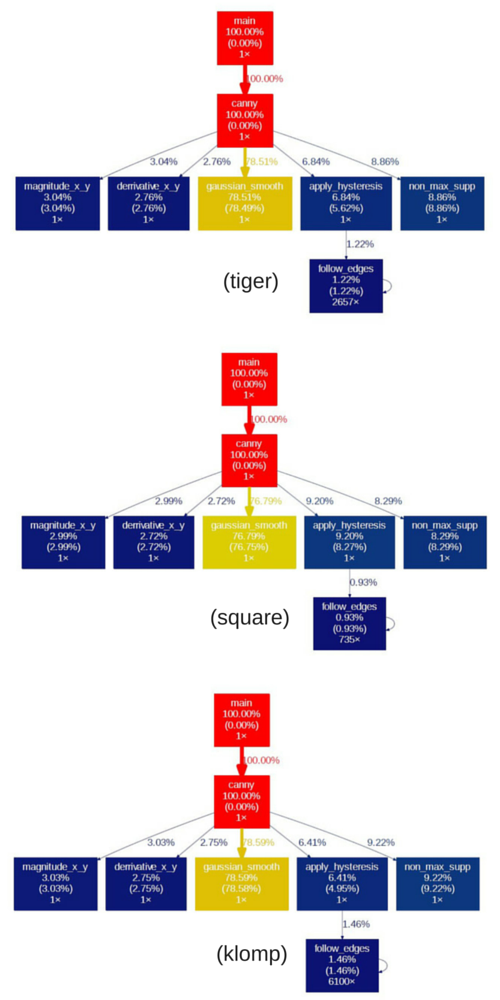
\includegraphics[width=0.4\textwidth]{pic/mix3.png}
\caption{Complexity of canny edge program with tiger.pgm, square.pgm, and klomp.pgm as input files}
\label{fig:profile}
\end{figure} 

Moreover, according to the control flow graph which is seen in Figure \ref{fig:profile2}, there are several steps performed in canny edge program: 1) Convolve the image with a separable gaussian filter. 2) Take the dx and dy the first derivatives. 3) Compute the magnitude. 4) Perform non-maximal suppression. 5) Perform hysteresis. The most complex function (i.e. gaussian\_smooth), is performed in the first step which gives the value that is used in another procedure (derivative\_x\_y). This condition makes us easy to split the computation in two separated resources in parallel, then the result of the computation is merged. However, further investigation to the gaussian-smooth function revealed that this function performs the blurring process in two step, x-direction and y-direction as seen in Figure~\ref{fig:convol}. These two steps are not independent; the y-direction process uses x-direction result as the input. Therefore, we cannot do the computation in parallel (using two sperated resources: DSP and NEON) by separating these two blurring steps. The distribution can be done by dividing the image into two part and then blur these two parts separately. 

\begin{figure}[!ht]
	    \centering
	    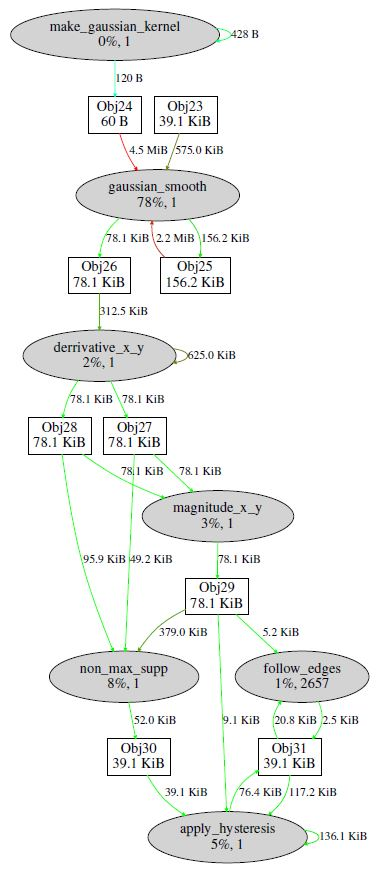
\includegraphics[width=0.4\textwidth]{pic/com_tiger.JPG}
   	\caption{Control Flow Graph of canny edge program with tiger.pgm as input file}
   	\label{fig:profile2}
   \end{figure} 

\begin{figure}[!ht]
    \centering
    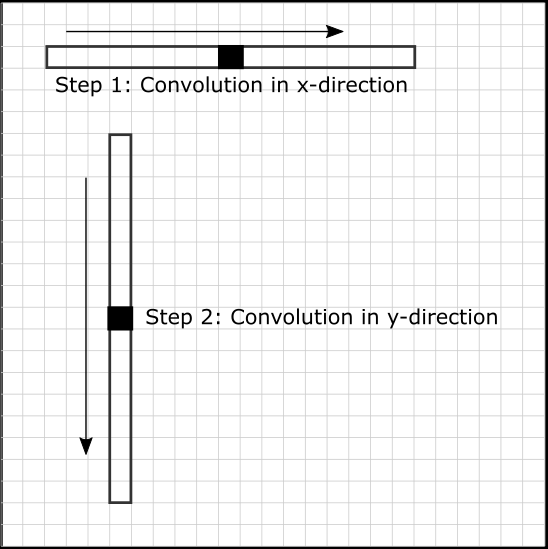
\includegraphics[width=0.35\textwidth]{pic/convol}
   \caption{Convolution process on x and y direction}
   \label{fig:convol}
\end{figure}

\subsubsection{Feature and Resource limitation}
To implement the canny edge algorithm on the Beagleboard, the features like DSP and NEON that is available on the Beagleboard must be well utilized. In addition, hardware limitation such as the available memory size for a memory pool, and communication overhead has to be complied.

Beagleboard features dedicated DSP TMS320C64x family, and NEON on the GPP that can perform vector multiplication. Both features, the DSP and NEON, can be exploited for the parallel computation. However, the dedicated DSP cannot perform floating point operation in nature, so the floating point operation is converted into fixed point operation.

The available memory size for a memory pool that can be used in total is 851968 bytes. Because of the DSP is not as well protected as the GPP to illegal writes, writing to memory outside the allocated area can have unexpected results. We can avoid this problem by minimizing the size of the allocated shared memory. We only provide the buffer size as large as the image that is needed by DSP, so that we only copy a certain part of the image to the shared memory. 

The communication overhead appeared in pool notify protocol which is used to perform data sharing between GPP and DSP. The initialization of this protocol has averagely constant execution time that may create major disadvantage especially when small size picture is processed. In this case, the parallel calculation does not give any advantages compare to overhead caused by communication. 

\subsubsection{Compiler options}
There are several compiler options in makefile that were used so that the Beagleboard features such as DSP and NEON can be used as follows:
\begin{itemize}
\item -O3: This optimization provides the highest level of optimization of code for the execution time and code size.
\end{itemize}
\begin{itemize}
\item -march=armv7-a: This specifies the name of the target is armv7-a architecture. It determines assembly code that is produced.
\end{itemize}
\begin{itemize}
\item -mtune=cortex-a8: This option specifies the target ARM processor for which GCC should tune the performance of the code is cortex-a8.
\end{itemize}
\begin{itemize}
\item -mfpu=neon: This specifies the floating-point hardware being used is NEON extension.
\end{itemize}
\begin{itemize}
\item -mfloat-abi=softfp: Specifies floating-point ABI to use is ‘softfp’. It allows us to use hardware floating-point instructions, but still uses the soft-float calling conventions.
\end{itemize}
\begin{itemize}
\item -ftree-vectorize: This option enable the vectorization.
\end{itemize}
\begin{itemize}
\item -ffast-math: This option enable vectorization of floating point reductions.
\end{itemize}

\section{Solution and implementation}
% Here we answer the question stated n the problem statement
To implement the canny edge program on the Beagleboard, there are several steps performed as seen in Figure \ref{fig:timingdiagram}: Read the PGM image, established the communication between DSP and GPP, perform gaussian-smooth function in DSP and NEON in parallel, combine the result of parallel calculation, and perform the rest of canny edge detection algorithm. At the end of the program, a procedure to verify the result (calculate the error and write the error output) is added.

The major speed up is expected to be obtained by optimizing both the gaussian-smooth function and communication process between DSP and GPP.     

\begin{figure}[!ht]
    \centering
    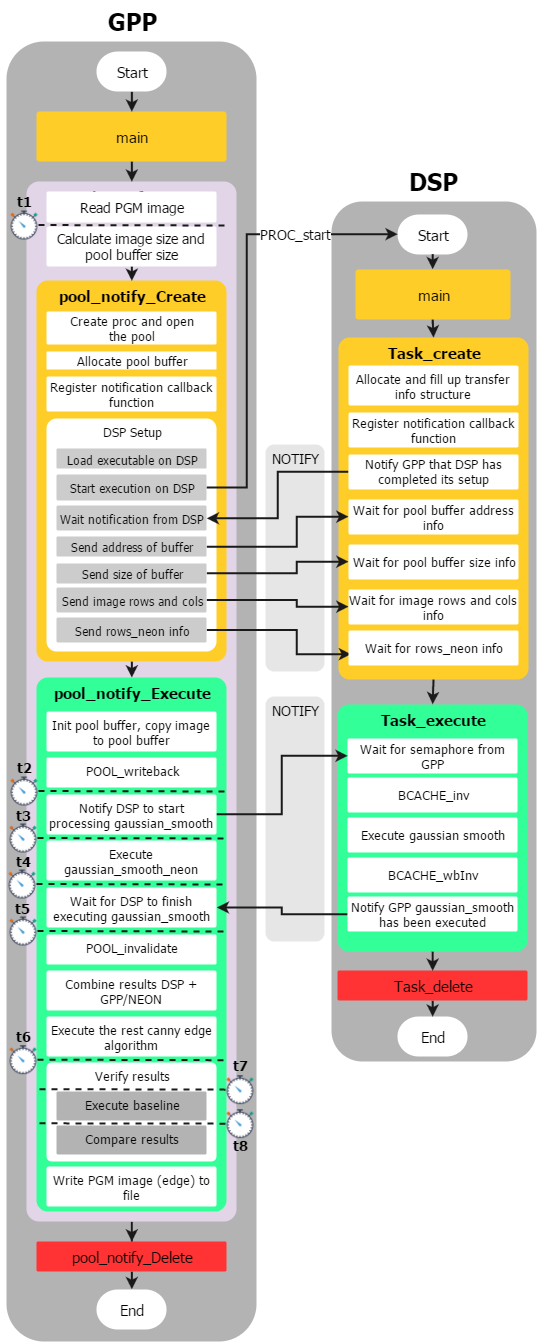
\includegraphics[width=0.45\textwidth]{pic/timing_diagram.png}
   \caption{Flow diagram of the proposed solution}
   \label{fig:timingdiagram}
\end{figure} 


% \subsection{Fixed point on gaussian-smooth function}
% \textbf{will be filled by Angga}

\subsection{GPP-DSP communication}
To perform data sharing between GPP and DSP, pool-notify protocol \cite{paper2} has been used. The protocol utilizes shared memory pool to store the data that can be accessed (written/read) by the GPP and DSP. This protocol is done by 3 main functions in GPP: pool\_notify\_Create, pool\_notify\_Execute, and pool\_notify\_Delete which release the allocated resources, and DSP: Task\_create, Task\_execute, and Task\_delete.

\subsubsection{GPP}
In pool\_notify\_Create function, the resources which are used by the pool\_notify are allocated and initialized. Also, in this function GPP send notifications to the DSP with information about the address of the control structure, and data buffer to be used by the application. The function is started with PROC module creation and setting by calling PROC\_setup and PROC\_attach, which is used to boot-load the DSP. After that, a POOL is opened with the configuration related to the size of the shared memory between the DSP and GPP, followed by the data buffer allocation which will be used by the protocol, which is done by POOL\_alloc function. If the data buffer is succesfully allocated, the shared memory address obtained from POOL\_alloc is then translated into specific address which can be read by DSP using POOL\_translateAddr function. Basicaly, after the DSP application setup is successfully created in GPP side, it is loaded to DSP by calling PROC\_load, and the DSP is started after PROC\_start is called. The GPP then wait the confirmation from the DSP before continuing to the next step, indicated by sem\_wait. Once the notification is received by the GPP, the GPP sends the information needed by the DSP to performs the calculation in 4 consecutive NOTIFY\_notify messages: the address of the allocated buffer on the shared memory, the size of the allocated buffer on the shared memory, image size to DSP (rows and cols), and rows\_neon that informs which rows the DSP must start (for load sharing purpose). The size of the allocated buffer on the shared memory depends on the size of the part of the image that will be handled by the DSP so that we can minimize the size of allocated buffer on shared memory and also minimize the write or read action to this shared memory. 

The pool\_notify\_Execute implements the execution phase. This function is started by executing unit\_init which fills the DSP buffer with the image data, followed by POOL\_writeback calls. Then, smoothedIm pointer is reserved with malloc function to save the result of the gaussian-smooth computation. GPP notifies the DSP to start process the gaussian-smooth function with NOTIFY\_notify message, then wait the DSP to finish the computation with sem\_wait, invalidate the content of the buffer with POOL\_invalidate, and copy the content of the buffer to smoothedIm using memcopy.

The pool\_notify\_Delete releases the allocated resources. This function begins by putting DSP in local reset with PROC\_stop, unregister the earlier registered event using NOTIFY\_unregister, and followed by POOL\_free which release the memory which is allocated for the data buffer. Then POOL\_close is called to lose the pool and makes it unavailable to DSP. Finally, the resources used by the PROC module is released using PROC\_detach, and the PROC module is destroyed using PROC\_destroy. This procedure also releases all allocated resources on the GPP-side of DSPLINK.

\subsubsection{DSP}
After in GPP side calls PROC\_start, the DSP starts initializing and obtaining cache align size by first executing DSPLINK\_init, and DSPLINK\_ALIGN before calling Task\_create function. In Task\_create function, the resources needed by the DSP are prepared. This function allocates and initialized Task\_TransferInfo structure, register notification for the event callback to get control and data buffer pointers from the GPP-side, and send the notification to the GPP side using NOTIFY\_notify message indicating that the setup is successfully done. The DSP then wait for the event callback from the GPP-side to post the semaphore indicating receipt of the data buffer pointer, buffer size, image width and height, and number of rows processed by NEON using SEM\_pend.

In Task\_execute function, the function waiting for the notification from the GPP side to start the gaussian-smooth computation using SEM\_pend. Once the notification is received, specified memory range in the cache is invalidated using BCACHE\_inv \cite{paper3}, the gaussian-smooth is computed, and the cache is written back (also invalidated) using BCACHE\_wbInv \cite{paper3}. The DSP then notifies the GPP using NOTIFY\_notify message to indicate that the calculation is finished.

Task\_delete function, notification for the event callback used to get control and data buffer pointers from the GPP-side is unregistered using NOTIFY\_unregister, and The memory used to store the inforation structure is cleaned using MEM\_free.

% \begin{figure}[!ht]
% 	    \centering
% 	    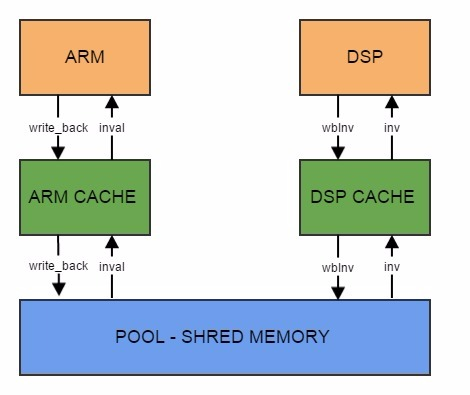
\includegraphics[width=0.4\textwidth]{pic/comm.jpg}
%   	\caption{ Write data into and read data from POOL}
%   	\label{fig:communication}
%   \end{figure} 
   

\subsection{Gaussian-smooth function in DSP and NEON}
Both of gaussian-smooth function in DSP and NEON are implemented by using fixed-point operation which introduces a small error as a trade-off of improving the execution time. In the DSP, fixed-point operation is implemented using a kernel with the Q17 format and fixed-point operation in NEON is implemented using Q16 kernel format. The constant value of sigma allows us to use pre-generated kernel array because of the unchanged windowsize, center value, and kernel function. Improvement is done by designing and testing the implementation on DSP and NEON separately at first, and then balancing the load to minimize the synchronization time hence the optimal improvement can be obtained. 

\subsubsection{NEON}
NEON is a combined 64-bit and 128-bit SIMD instruction set that provides standardized acceleration for media and signal processing applications. Gaussian-smooth improvement in NEON is done by utilizing 128-bit Quad-word register for vector multiplication. The modification of image array and kernel array have to be made, so that it is suitable for vector processing. 

The image pixel modification is done by adding 16 additional pixels to simplify the edge case. Eight pixels are added both on the left-side and the right-side of the image for the blurring process in the x-direction. For the blurring process in the y-direction, eight pixels are added at the top and bottom part of the image. By performing the modification, the same NEON instruction for multiplication can be implemented without having to check the edge case and changing the result of the blurring process. 

Moreover, kernel modification is done by adding two zeros as the first and the last element of the array as shown by Figure \ref{fig:kernel_mod}. The kernel size is then changed to 17, so that 17 multiplication for each of blurring process for one pixel has to be done. The multiplication operation is done by two ways, first using the NEON instruction for 16 neighbor multiplication, and standard arithmetic multiplication operation to get the gaussian multiplication of the center pixel. 

\begin{figure}[!ht]
	    \centering
	    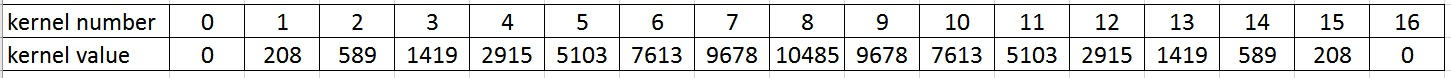
\includegraphics[width=0.5\textwidth]{pic/kernel.jpg}
   	\caption{New kernel array after modification}
   	\label{fig:kernel_mod}
   \end{figure}

For Q16 kernel format, Quad-word register to stored 4x32 bit data is utilized so that the calculation for four data can be done at the same time. While calculating gaussian smooth for one pixel, kernel and its eight neighbor pixels on both left and right side are multiplied. The calculation is finished in four NEON calculation periods. The multiplication of center pixel with its corresponding kernel value in the end is done separately. The last step is accumulating all the multiplication result and normalize it by dividing the accumulation with the sum of the kernel value.

We also tried to implement the Q8 format kernel fixed-point operation. It utilizes Quad-word register to store 8x16 bit data. Eight multiplication can be done at the same time and the 16 neighbor pixel is finished in 2 periods of NEON multiplication instruction. The trade-off is the kernel which is used has less precision and the accumulation of the results is finished after eight extractions and summation operation.

In addition to these two fixed-point implementation, we also tried to use NEON floating-point operation to compare it with the fixed-point operation.

\subsubsection{DSP}
The DSP in OMAP3530 (TMS320C64x+) is not well suited for floating point operations. It only supports fixed-point operations in nature. To be able to achieve a significant speedup, the Gaussian smooth function was modified to use fixed-point. Implementing the fixed-point on DSP is much faster than floating point. Considering the degree of precision and overflow condition, the pre-generated kernel in Q17 format is chosen. The multiplication between kernel and image pixel is then stored in 32-bit unsigned integer. The maximum result of the accumulated multiplication can be handled by 32-bit unsigned integer, and the bigger value of Q-format ten can be chosen. However, the blur-boosting step in y-direction blurring process may causes overflow condition.

\textit{Load-Sharing}: To accelerate the gaussian-smooth function, the load is distributed and the gaussian smooth in DSP and GPP is performed in parallel. Tthe image is partitioned into 2, the upper and lower part. The upper part is processed by NEON and the lower part is processed by DSP. Because of the gaussian smoothing algorithm in nature uses neighbor pixels to blurr the respective center pixel, the image cannot be simpl partitioned, separately processed, and combined later. It will raise the problem at the separation boundary. For the upper part, the next 8 pixels should also be included (half side size of the modified kernel) to perform the valid gaussian smoothing for the last line pixel. For the lower part, the previous 8 pixels should be included to perform valid gaussian smoothing for first-row pixel. This step is demonstrated by Figure \ref{fig:divide et impera}. the optimal load sharing is obtained by dividing the image with 38:62 ratio, for NEON and DSP respectively.
% Reference Guide

\begin{figure}[!ht]
	    \centering
	    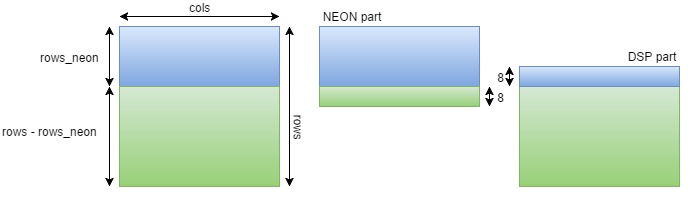
\includegraphics[width=0.5\textwidth]{pic/row_col.jpg}
   	\caption{Image separation ilustration for load sharing}
   	\label{fig:divide et impera}
   \end{figure}


\subsection{Profiling solutions}
Profiling the proposed solutions are performed by using timers inside the source code instead of using MCPROF as it is intended to work on Intel processor rather than ARM. Execution time of the application in certain areas is extracted during profiling. The detailed characteristic of the timers, which indicates the starting point and finishing point, can be seen in Figure~\ref{fig:timingdiagram}. 

In Figure~\ref{fig:timingdiagram}, the total execution time of the proposed solutions start from t1 until t6, whereas the total execution time of the baseline start from t7 until t8. In order to give more detailed result, the total execution time is split into several parts. The first part is allocation time, which start from t1 until t2. The allocation time represents the time nedded for setting up the GPP and DSP before executing canny edge algorithm. The second part is canny edge algorithm execution time, which start from t2 until t6. In addition, this part can be split into several parts, namely DSP time and NEON time, starting from t2 until t5 and t3 until t4 respectively. As the DSP and NEON execute the gaussian smooth function in parallel, the longest time between DSP and NEON execution time will be used to calculate the total execution time.

The DSP time, NEON time, and total execution time are useful for calculating the speedup of our proposed solutions. The calculation and analysis of speedup will be explained in the next section.

%\subsubsection{Other calculation on NEON}

%\subsection{The Communication}

%\subsection{Memory Limitation}
%\subsection{Optimizations for DSP,ARM,and NEON}
%\subsection{Compiler Options}


\section{Result analysis and comparison}

\subsection{NEON fixed-point U16 vs. fixed-point U32 vs. floating-point}

At first, the execution time and speed up for canny edge implementation using NEON only was compared. The optimum solution is chosen to be used in the operation used in load sharing process.

The comparison of different data-type being used on NEON implementation is shown by Table \ref{gaustotal}. Two different kinds of speed up, speed up of gaussian smooth function and speed up of the total execution time were calculated. U16 means that we are using Quad-word register as 8x16 bit data register while U32 means that Quad-word register was used as 4x32 bit data register.

\begin{table*}[!ht]
\centering
\caption{The execution times measured in $\mu$s and Speedup
for Gaussian and Total for the different data types operation (NEON 100\%)}
\label{gaustotal}
\begin{tabular}{|c|l|c|c|c|c|c|c|c|c|c|}
\hline
\multicolumn{11}{|c|}{\textbf{GAUSSIAN}} \\ \hline
\multicolumn{2}{|c|}{\textbf{PICTURE}} & \multicolumn{3}{c|}{\textbf{TIGER}} & \multicolumn{3}{c|}{\textbf{KLOMP}} & \multicolumn{3}{c|}{\textbf{SQUARE}} \\ \hline
\multicolumn{2}{|l|}{} & \textbf{Baseline} & \textbf{\begin{tabular}[c]{@{}c@{}}NEON\end{tabular}} & \textbf{SpeedUp} & \textbf{Baseline} & \textbf{\begin{tabular}[c]{@{}c@{}}NEON\end{tabular}} & \textbf{SpeedUp} & \textbf{Baseline} & \textbf{\begin{tabular}[c]{@{}c@{}}NEON\end{tabular}} & \textbf{SpeedUp} \\ \hline
\multicolumn{1}{|l|}{\textbf{NEON}} & \textbf{U16} & 78277.5 & 20722 & 3.77855 & 165268 & 44830 & 3.68615 & 30105 & 7888.5 & 3.81635 \\ \hline
\multicolumn{1}{|l|}{\textbf{}} & \textbf{U32} & 76309.5 & 21408 & 3.56455 & 166488.5 & 47561.5 & 3.50225 & 29862 & 8499.5 & 3.5143 \\ \hline
\multicolumn{1}{|l|}{\textbf{}} & \textbf{FLOAT} & 76858.5 & 31692 & 2.42525 & 164657 & 65704.5 & 2.5057 & 29648 & 11688.5 & 2.53665 \\ \hline
\multicolumn{11}{|c|}{\textbf{TOTAL}} \\ \hline
\multicolumn{2}{|c|}{\textbf{PICTURE}} & \multicolumn{3}{c|}{\textbf{TIGER}} & \multicolumn{3}{c|}{\textbf{KLOMP}} & \multicolumn{3}{c|}{\textbf{SQUARE}} \\ \hline
\multicolumn{2}{|c|}{} & \textbf{Baseline} & \textbf{Total} & \textbf{SpeedUp} & \textbf{Baseline} & \textbf{Total} & \textbf{SpeedUp} & \textbf{Baseline} & \textbf{Total} & \textbf{SpeedUp} \\ \hline
\textbf{NEON} & \multicolumn{1}{c|}{\textbf{U16}} & 107941 & 50690.5 & 2.1294 & 230256 & 113221 & 2.03375 & 39994 & 18432.5 & 2.16975 \\ \hline
\textbf{} & \multicolumn{1}{c|}{\textbf{U32}} & 104691 & 51269.5 & 2.04195 & 235413 & 116059 & 2.0287 & 39628 & 19013 & 2.08425 \\ \hline
\textbf{} & \multicolumn{1}{c|}{\textbf{FLOAT}} & 105515 & 66879 & 1.5842 & 232742 & 132523 & 1.7563 & 39352 & 22110 & 1.77985 \\ \hline
\end{tabular}
\end{table*}

\begin{figure}[!ht]
    \centering
    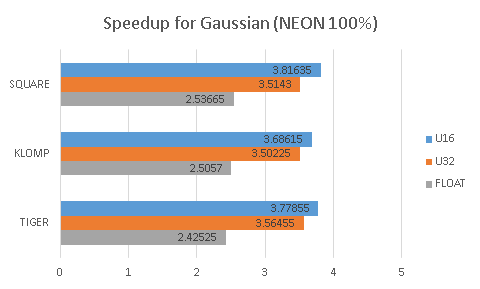
\includegraphics[width=0.45\textwidth]{pic/uneon}
   \caption{Speedup for gaussian smooth (NEON 100\%)}
   \label{fig:speedupneononly}
\end{figure}


\begin{table}[!ht]
\centering
\caption{The execution times measured in  $\mu$s and Speedup for Gaussian (NEON 50\% DSP 50\%)}
\label{gauss50}
\begin{tabular}{|l|c|c|c|c|}
\hline
\multicolumn{5}{|c|}{\textbf{Gaussian(NEON 50\% DSP 50\%)}}                                                                       \\ \hline
\multicolumn{1}{|c|}{\textbf{Pic.}} & \textbf{Baseline} & \textbf{DSP} & \textbf{NEON} & \textbf{Speedup} \\ \hline
Tiger                                   & 81878.7           & 7751.3      & 11067.7        & 7.398          \\ \hline
Klomp                                   & 171183          & 15177.7      & 23804       & 7.192          \\ \hline
Square                                  & 31178.7           & 3011       & 4649        & 6.707          \\ \hline
\end{tabular}
\end{table}

\begin{table}[!ht]
\centering
\caption{The execution times measured in  $\mu$s and Speedup for Total (NEON 50\% DSP 50\%)}
\label{total50}\begin{tabular}{|l|c|c|c|c|l|}
\hline
\multicolumn{6}{|c|}{\textbf{Total (NEON 50\% DSP 50\%)}}                                                                                                                                                                                \\ \hline
\textbf{Pic.} & \multicolumn{1}{l|}{\textbf{Baseline}} & \textbf{\begin{tabular}[c]{@{}c@{}}Canny \\ Edge\\  Algorithm\end{tabular}} & \textbf{Overhead} & \textbf{\begin{tabular}[c]{@{}c@{}}Speedup\\ with \\ Over \\ head\end{tabular}} & \multicolumn{1}{c|}{\textbf{\begin{tabular}[c]{@{}c@{}}Speedup \\ without \\ Over \\ head\end{tabular}}} \\ \hline
Tiger             & 109202                               & 41850                                                                       & 23752.7           & 1.67                                                                     & 2.61                                                                                              \\ \hline
Klomp             & 232024.7                               & 94197.7                                                                     & 21321.7           & 2.02                                                                     & 2.48                                                                                              \\ \hline
Square            & 40222.3                                & 15879.3                                                                     & 22929          & 1.04                                                                     & 2.54                                                                                              \\ \hline
\end{tabular}
\end{table}

The result shows that floating point operation has the lowest value both on total speed up or gaussian smooth speed, as is shown in Figure \ref{fig:speedupneononly} . Moreover, the total speed up of the floating point operation is below 2 while both of fixed-point operation surpass the minimum requirement speed up of 2. The U16 format gives a slightly bigger speed up. However, considering that the degree of precision being used at U16 is very low, we decided to use U32 format for the load sharing step so that the risk of producing the result with a bigger error is minimized.

\subsection{Load Balancing and Speedup}

Several ratio for balancing the load between NEON and DSP are tested. the testing was started from ratio 1:1. The execution time and speed up for gaussian-smooth and the overall execution time were both measured separately. The balance condition was observed solely from the gaussian smooth execution time because this is the function that  executed in parallel by NEON and DSP. The result of 1:1 load ratio are shown by Table \ref{gauss50} and Table \ref{total50}. For the Gaussian-smooth, the speed up is chosen based on the slower achievement between the two:
\begin{equation*}
\text{Gaussian Speed up} = \frac{\text{Execution Time of Baseline Gaussian}}{\text{max(DSP, NEON)}}        
\end{equation*}

While the total speed up is calculated as : 
\begin{equation*}
\text{Total Speed up} = \frac{\text{Execution Time of Baseline Canny}}{\text{Execution Time of Optimized Canny}}        
\end{equation*}

As seen in Table \ref{gauss50}, DSP performed faster gaussian-smooth computation for the same amount of load. We had to increase the DSP load until the NEON gaussian-smooth computation time is the same with DSP gaussian-smooth computation time.     

The load ratio result of 37:63 are shown by Table \ref{gauss37} and Table \ref{total37}. The results show that the DSP gaussian-smooth execution time was slightly bigger than NEON, so we had to reduce the DSP partition a little bit. The next test used load ratio of 38:62. 

\begin{table}[!ht]
\centering
\caption{The execution time measured in  $\mu$s and Speed up for Gaussian (NEON 37\% DSP 63\%)}
\label{gauss37}
\begin{tabular}{|l|c|c|c|c|}
\hline
\multicolumn{5}{|c|}{\textbf{Gaussian(NEON 37\% DSP 63\%)}}                                                                       \\ \hline
\multicolumn{1}{|c|}{\textbf{Pic.}} & \textbf{Baseline} & \textbf{DSP} & \textbf{NEON} & \textbf{Speedup} \\ \hline
Tiger                                   & 79303.2           & 10061.7      & 8630.6        & 7.88153          \\ \hline
Klomp                                   & 162896.7          & 19818.1      & 18133.6       & 8.22195          \\ \hline
Square                                  & 29794.3           & 3897.2       & 3454.7        & 7.64525          \\ \hline
\end{tabular}
\end{table}

\begin{table}[!ht]
\centering
\caption{The execution time measured in  $\mu$s and Speedup for Total (NEON 37\% DSP 63\%)}
\label{total37}
\begin{tabular}{|l|c|c|c|c|l|}
\hline
\multicolumn{6}{|c|}{\textbf{Total (NEON 37\% DSP 63\%)}}                                                                                                                                                                                \\ \hline
\textbf{Pic.} & \multicolumn{1}{l|}{\textbf{Baseline}} & \textbf{\begin{tabular}[c]{@{}c@{}}Canny \\ Edge\\  Algorithm\end{tabular}} & \textbf{Overhead} & \textbf{\begin{tabular}[c]{@{}c@{}}Speedup\\ with \\ Over \\ head\end{tabular}} & \multicolumn{1}{c|}{\textbf{\begin{tabular}[c]{@{}c@{}}Speedup \\ without \\ Over \\ head\end{tabular}}} \\ \hline
Tiger             & 108792.2                               & 42697                                                                       & 22958.4           & 1.66596                                                                     & 2.54819                                                                                              \\ \hline
Klomp             & 228967.5                               & 97482.4                                                                     & 24176.1           & 1.88657                                                                     & 2.35316                                                                                              \\ \hline
Square            & 39968.8                                & 15606.8                                                                     & 21652.2           & 1.10265                                                                     & 2.56107                                                                                              \\ \hline
\end{tabular}
\end{table}

The load ratio result of 38:62 are shown by Table \ref{gauss38} and Table \ref{total38}. The difference between NEON and DSP gaussian-smooth execution time was smaller. The results also show that for some image the NEON gaussian-smooth execution time was smaller than DSP execution time and for another image the NEON execution time was bigger. Hence we chose this ratio as the optimal load sharing ratio.

\begin{table}[!ht]
\centering
\caption{The execution time measured in  $\mu$s and Speedup for Gaussian (NEON 38\% DSP 62\%)}
\label{gauss38}
\begin{tabular}{|l|c|c|c|c|}
\hline
\multicolumn{5}{|c|}{\textbf{Gaussian (NEON 38\% DSP 62\%)}}                                                                       \\ \hline
\multicolumn{1}{|c|}{\textbf{Pictures}} & \textbf{Baseline} & \textbf{DSP} & \textbf{NEON} & \textbf{Speedup} \\ \hline
Tiger                                   & 78412           & 9637.2      & 8892.6        & 8.136          \\ \hline
Klomp                                   & 166772.4          & 18823.2      & 19030.8       & 8.763          \\ \hline
Square                                  & 29559.4           & 3704.4       & 3680.4        & 7.979          \\ \hline
\end{tabular}
\end{table}


\begin{table}[!ht]
\centering
\caption{The execution time measured in  $\mu$s and Speed up for Total (NEON 38\% DSP 62\%)}
\label{total38}
\begin{tabular}{|l|c|c|c|c|l|}
\hline
\multicolumn{6}{|c|}{\textbf{Total (NEON 38\% DSP 62\%)}}                                                                                                                                                                                                                                                                                                \\ \hline
\textbf{Pic.} & \multicolumn{1}{l|}{\textbf{Baseline}} & \textbf{\begin{tabular}[c]{@{}c@{}}Canny \\ Edge\\  Algorithm\end{tabular}} & \textbf{Overhead} & \textbf{\begin{tabular}[c]{@{}c@{}}Speedup\\ with \\ Over \\ head\end{tabular}} & \multicolumn{1}{c|}{\textbf{\begin{tabular}[c]{@{}c@{}}Speedup \\ without \\ Over \\ head\end{tabular}}} \\ \hline
Tiger             & 108013.8                               & 42358.2                                                                       & 16797.2           & 1.8278                                                                     & 2.55114                                                                                              \\ \hline
Klomp             & 236358.4                               & 91027.8                                                                    & 21130.4           & 2.10958                                                                     & 2.59682                                                                                              \\ \hline
Square            & 39538.4                                & 15380.8                                                                     & 17199.8           & 1.2271                                                                     & 2.57068                                                                                              \\ \hline
\end{tabular}
\end{table}

As seen in Table \ref{gauss38}, the gaussian-smooth function speed up of all test image are around 8. We managed to run the optimized canny edge algorithm up to 2.59 times faster than baseline if we did not include the communication overhead. If the communication overhead on optimized canny total time was also included, the speed up more than 2 was only attained by the biggest image, Klomp.pgm. The smaller the image size, the less the effect of optimization on gaussian-smooth function. As seen in Table \ref{total38}, square image as the smallest image, only achieved 1.2 times speed up although its gaussian smooth speedup was almost 8. The execution time for establishing the communication protocol was much bigger than the gaussian smooth execution time for the small image case. Figure~\ref{fig:speedupfig} gives more sophisticated view for comparing the total execution time of different configurations.

\begin{figure}[!ht]
\centering
\begin{subfigure}[b]{0.4\textwidth}
    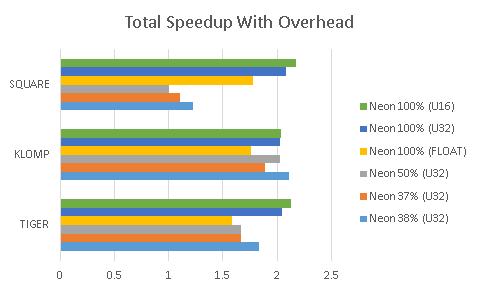
\includegraphics[width=\textwidth]{pic/totalspeedupOv}
    \caption{}
    \label{fig:speedov}
\end{subfigure}
\begin{subfigure}[b]{0.4\textwidth}
    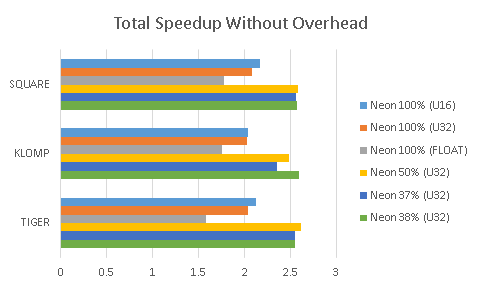
\includegraphics[width=\textwidth]{pic/totalspeedupwOv}
    \caption{}
    \label{fig:speedwov}
\end{subfigure}
   \caption{Total speed up: (a) with overhead, and (b) without overhead}
   \label{fig:speedupfig}
\end{figure} 

\subsection{Error Analysis}
The use of fixed-point in the optimized solution introduces some slight inaccuracies. Large inaccuracies can be seen obviously, but for small inaccuracies we need more sophisticated method to quantify the differences. Therefore, it is required to do error analysis for verifying the results.

\begin{table}[!ht]
\centering
\caption{Error Comparison}
\label{errorcompar}
\begin{tabular}{ccccccc}
\hline
\multicolumn{1}{|c|}{\textbf{Pic.}} & \multicolumn{3}{c|}{\textbf{NEON 50\% and DSP 50\%}} & \multicolumn{3}{c|}{\textbf{NEON 37\% and DSP 63\%}} \\ \hline
\multicolumn{1}{|c|}{} & \multicolumn{1}{c|}{\begin{tabular}[c]{@{}c@{}}False \\ alarm \\ (\%)\end{tabular}} & \multicolumn{1}{c|}{\begin{tabular}[c]{@{}c@{}}Mis\\ detection\\  (\%)\end{tabular}} & \multicolumn{1}{c|}{\begin{tabular}[c]{@{}c@{}}Total\\  Error \\ (\%)\end{tabular}} & \multicolumn{1}{c|}{\begin{tabular}[c]{@{}c@{}}False \\ alarm\\  (\%)\end{tabular}} & \multicolumn{1}{c|}{\begin{tabular}[c]{@{}c@{}}Mis\\ detection \\ (\%)\end{tabular}} & \multicolumn{1}{c|}{\begin{tabular}[c]{@{}c@{}}Total \\ Error \\ (\%)\end{tabular}} \\ \hline
\multicolumn{1}{|c|}{Tiger} & \multicolumn{1}{c|}{0.18} & \multicolumn{1}{c|}{0.135} & \multicolumn{1}{c|}{0.315} & \multicolumn{1}{c|}{0.18} & \multicolumn{1}{c|}{0.14} & \multicolumn{1}{c|}{0.32} \\ \hline
\multicolumn{1}{|c|}{Klomp} & \multicolumn{1}{c|}{0.6184} & \multicolumn{1}{c|}{0.27864} & \multicolumn{1}{c|}{0.89713} & \multicolumn{1}{c|}{0.665365} & \multicolumn{1}{c|}{0.2903} & \multicolumn{1}{c|}{0.9557} \\ \hline
\multicolumn{1}{|c|}{Square} & \multicolumn{1}{c|}{0.48611} & \multicolumn{1}{c|}{0.47222} & \multicolumn{1}{c|}{0.95833} & \multicolumn{1}{c|}{0.486111} & \multicolumn{1}{c|}{0.4722} & \multicolumn{1}{c|}{0.9583} \\ \hline
 &  &  &  &  &  &  \\ \hline
\multicolumn{1}{|c|}{\textbf{Pic.}} & \multicolumn{3}{c|}{\textbf{NEON 38\% and DSP 62\%}} & \multicolumn{3}{c|}{\textbf{NEON U16}} \\ \hline
\multicolumn{1}{|c|}{} & \multicolumn{1}{c|}{\begin{tabular}[c]{@{}c@{}}False\\  alarm\\  (\%)\end{tabular}} & \multicolumn{1}{c|}{\begin{tabular}[c]{@{}c@{}}Mis\\ detection\\  (\%)\end{tabular}} & \multicolumn{1}{c|}{\begin{tabular}[c]{@{}c@{}}Total \\ Error\\  (\%)\end{tabular}} & \multicolumn{1}{c|}{\begin{tabular}[c]{@{}c@{}}False\\  alarm\\  (\%)\end{tabular}} & \multicolumn{1}{c|}{\begin{tabular}[c]{@{}c@{}}Mis\\ detection \\ (\%)\end{tabular}} & \multicolumn{1}{c|}{\begin{tabular}[c]{@{}c@{}}Total \\ Error\\  (\%)\end{tabular}} \\ \hline
\multicolumn{1}{|c|}{Tiger} & \multicolumn{1}{c|}{0.18} & \multicolumn{1}{c|}{0.14} & \multicolumn{1}{c|}{0.32} & \multicolumn{1}{c|}{0.1675} & \multicolumn{1}{c|}{0.1875} & \multicolumn{1}{c|}{0.355} \\ \hline
\multicolumn{1}{|c|}{Klomp} & \multicolumn{1}{c|}{0.66536} & \multicolumn{1}{c|}{0.29036} & \multicolumn{1}{c|}{0.95572} & \multicolumn{1}{c|}{0.255208} & \multicolumn{1}{c|}{0.7239} & \multicolumn{1}{c|}{0.9791} \\ \hline
\multicolumn{1}{|c|}{Square} & \multicolumn{1}{c|}{0.48611} & \multicolumn{1}{c|}{0.47222} & \multicolumn{1}{c|}{0.95833} & \multicolumn{1}{c|}{0.486111} & \multicolumn{1}{c|}{0.4722} & \multicolumn{1}{c|}{0.9583} \\ \hline
 &  &  &  &  &  &  \\ \hline
\multicolumn{1}{|c|}{\textbf{Pic.}} & \multicolumn{3}{c|}{\textbf{NEON U32}} & \multicolumn{3}{c|}{\textbf{FLOAT}} \\ \hline
\multicolumn{1}{|c|}{} & \multicolumn{1}{c|}{\begin{tabular}[c]{@{}c@{}}False \\ alarm \\ (\%)\end{tabular}} & \multicolumn{1}{c|}{\begin{tabular}[c]{@{}c@{}}Mis\\ detection\\  (\%)\end{tabular}} & \multicolumn{1}{c|}{\begin{tabular}[c]{@{}c@{}}Total \\ Error \\ (\%)\end{tabular}} & \multicolumn{1}{c|}{\begin{tabular}[c]{@{}c@{}}False \\ alarm \\ (\%)\end{tabular}} & \multicolumn{1}{c|}{\begin{tabular}[c]{@{}c@{}}Mis\\ detection \\ (\%)\end{tabular}} & \multicolumn{1}{c|}{\begin{tabular}[c]{@{}c@{}}Total \\ Error \\ (\%)\end{tabular}} \\ \hline
\multicolumn{1}{|c|}{Tiger} & \multicolumn{1}{c|}{0.175} & \multicolumn{1}{c|}{0.1375} & \multicolumn{1}{c|}{0.3125} & \multicolumn{1}{c|}{0} & \multicolumn{1}{c|}{0} & \multicolumn{1}{c|}{0} \\ \hline
\multicolumn{1}{|c|}{Klomp} & \multicolumn{1}{c|}{0.6992} & \multicolumn{1}{c|}{0.2812} & \multicolumn{1}{c|}{0.9804} & \multicolumn{1}{c|}{0} & \multicolumn{1}{c|}{0} & \multicolumn{1}{c|}{0} \\ \hline
\multicolumn{1}{|c|}{Square} & \multicolumn{1}{c|}{0.4861} & \multicolumn{1}{c|}{0.4791} & \multicolumn{1}{c|}{0.9652} & \multicolumn{1}{c|}{0} & \multicolumn{1}{c|}{0} & \multicolumn{1}{c|}{0} \\ \hline
\end{tabular}
\end{table}

Verification of the results comprises generation of the baseline and comparison between the optimized solution and the baseline by evaluating differences of all pixels. As the edge detection result only generated black color for the edge, which is represented as 0, and white color for the rest, which is represented as 255, it is quite straightforward to use only both values to calculate the error. The example of file comparison in hex format between the optimized solution and the baseline for the tiger image is depicted in Figure~\ref{fig:hexComparison}. From Figure~\ref{fig:hexComparison}, indeed, it is obvious that the pixels comprises only two values, 0x00 (0 or black) and 0xFF (255 or white).

\begin{figure}[!ht]
\centering
\begin{subfigure}[b]{0.24\textwidth}
    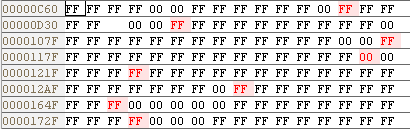
\includegraphics[width=\textwidth]{pic/baseline_hex}
    \caption{Baseline}
    \label{fig:baselineHex}
\end{subfigure}
\begin{subfigure}[b]{0.24\textwidth}
    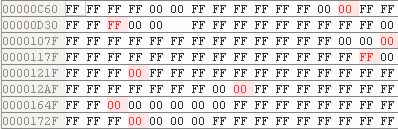
\includegraphics[width=\textwidth]{pic/optimal_hex}
    \caption{Optimized solution}
    \label{fig:optimizedHex}
\end{subfigure}
   \caption{Results comparison in hexadecimal}
   \label{fig:hexComparison}
\end{figure} 

The error rate comprises false-alarm detection and misdetection. False-alarm occurs when a black pixel appears in the area that is supposed to be white pixels according to the baseline. In contrast, misdetection occurs when a white pixel appears in the area that is supposed to be black pixels according to the baseline.

The visual difference between the optimal solution (38\% NEON and 62\% DSP using uint32 fixed-point) and the baseline is depicted in Figure~\ref{fig:tigerComparison}. The complete list of error rate can be seen in Table~\ref{errorcompar}.

%For instance, if the edge is detected in the x,y pixel inoptimized solution    

\begin{figure}[!ht]
\centering
\begin{subfigure}[b]{0.2\textwidth}
    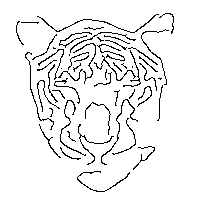
\includegraphics[width=\textwidth]{pic/tiger_baseline}
    \caption{Baseline}
    \label{fig:tigerBaseline}
\end{subfigure}
\begin{subfigure}[b]{0.2\textwidth}
    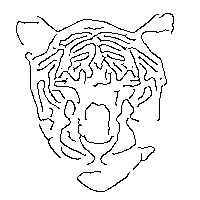
\includegraphics[width=\textwidth]{pic/tiger_38_u32_result}
    \caption{Optimal solution}
    \label{fig:tigerOptSol}
\end{subfigure}
\begin{subfigure}[b]{0.2\textwidth}
    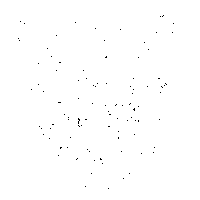
\includegraphics[width=\textwidth]{pic/tiger_38_u32_error}
    \caption{Differences}
    \label{fig:tigerDiffOptSol}
\end{subfigure}
   \caption{Results of edge detection applied to the tiger image}
   \label{fig:tigerComparison}
\end{figure} 

\section{Conclusion}
The Canny edge algorithm, when it is implemented on Beagleboard, can utilize its dedicated DSP and NEON features. The enhancement can be done by performing parallel computation using two separated resources, namely DSP and NEON, with load sharing mechanism and converting the floating point operation into the fixed-point operation. The speed up with the factor of 2.1, compared to the baseline canny edge detector program, was achieved by optimizing the heaviest function, i.e. gaussian-smooth.

There is a trade-off in floating point to fixed point operation conversion. When the floating point operation is converted into fixed point operation, some degree of precision is no longer considered so that it causes a few accuracy loss. In addition, a disadvantage is also found when using DSP, especially when small size of picture is processed due to its communication overhead takes considerably long execution time. For this project, the optimal load sharing ratio is 38:62, for NEON and DSP respectively.

% An example of a floating figure using the graphicx package.
% Note that \label must occur AFTER (or within) \caption.
% For figures, \caption should occur after the \includegraphics.
% Note that IEEEtran v1.7 and later has special internal code that
% is designed to preserve the operation of \label within \caption
% even when the captionsoff option is in effect. However, because
% of issues like this, it may be the safest practice to put all your
% \label just after \caption rather than within \caption{}.
%
% Reminder: the "draftcls" or "draftclsnofoot", not "draft", class
% option should be used if it is desired that the figures are to be
% displayed while in draft mode.
%
%\begin{figure}[!t]
%\centering
%\includegraphics[width=2.5in]{myfigure}
% where an .eps filename suffix will be assumed under latex, 
% and a .pdf suffix will be assumed for pdflatex; or what has been declared
% via \DeclareGraphicsExtensions.
%\caption{Simulation Results.}
%\label{fig_sim}
%\end{figure}

% Note that IEEE typically puts floats only at the top, even when this
% results in a large percentage of a column being occupied by floats.


% An example of a double column floating figure using two subfigures.
% (The subfig.sty package must be loaded for this to work.)
% The subfigure \label commands are set within each subfloat command,
% and the \label for the overall figure must come after \caption.
% \hfil is used as a separator to get equal spacing.
% Watch out that the combined width of all the subfigures on a 
% line do not exceed the text width or a line break will occur.
%
%\begin{figure*}[!t]
%\centering
%\subfloat[Case I]{\includegraphics[width=2.5in]{box}%
%\label{fig_first_case}}
%\hfil
%\subfloat[Case II]{\includegraphics[width=2.5in]{box}%
%\label{fig_second_case}}
%\caption{Simulation results.}
%\label{fig_sim}
%\end{figure*}
%
% Note that often IEEE papers with subfigures do not employ subfigure
% captions (using the optional argument to \subfloat[]), but instead will
% reference/describe all of them (a), (b), etc., within the main caption.


% An example of a floating table. Note that, for IEEE style tables, the 
% \caption command should come BEFORE the table. Table text will default to
% \footnotesize as IEEE normally uses this smaller font for tables.
% The \label must come after \caption as always.
%
%\begin{table}[!t]
%% increase table row spacing, adjust to taste
%\renewcommand{\arraystretch}{1.3}
% if using array.sty, it might be a good idea to tweak the value of
% \extrarowheight as needed to properly center the text within the cells
%\caption{An Example of a Table}
%\label{table_example}
%\centering
%% Some packages, such as MDW tools, offer better commands for making tables
%% than the plain LaTeX2e tabular which is used here.
%\begin{tabular}{|c||c|}
%\hline
%One & Two\\
%\hline
%Three & Four\\
%\hline
%\end{tabular}
%\end{table}


% Note that IEEE does not put floats in the very first column - or typically
% anywhere on the first page for that matter. Also, in-text middle ("here")
% positioning is not used. Most IEEE journals/conferences use top floats
% exclusively. Note that, LaTeX2e, unlike IEEE journals/conferences, places
% footnotes above bottom floats. This can be corrected via the \fnbelowfloat
% command of the stfloats package.






% conference papers do not normally have an appendix


% use section* for acknowledgement

\section*{Group member contribution}
As seen in Table \ref{contribution1} and Table \ref{contribution2}, in the first week, all group member assessed the problem formulation and create the to do list, then it was expanded into manpower assignment for each member. In week 2, the assessment was done for canny edge detector, NEON, DSP, and pool notify. In week 3, we concerned on the implementation of the canny edge algorithm in Beagleboard. In week 4, We worked on enhancement of the program to perform execution time speed up. In week 5, The result is collected and the program was tested, continued by report creation.
%
%The authors would like to thank...
%



% Please add the following required packages to your document preamble:
% \usepackage{multirow}
\begin{table*}[!ht]
\centering
\caption{Group member contribution week 1 - 3}
\label{contribution1}
\begin{tabular}{|l|l|l|c|l|c|}
\hline
\multicolumn{1}{|c|}{\multirow{2}{*}{\textbf{\begin{tabular}[c]{@{}c@{}}Group \\ Member\end{tabular}}}} & \multicolumn{2}{c|}{\textbf{Week 1}} & \textbf{Week 2} & \multicolumn{2}{c|}{\textbf{Week 3}} \\ \cline{2-6} 
\multicolumn{1}{|c|}{} & \multicolumn{1}{c|}{\textbf{Day 1}} & \multicolumn{1}{c|}{\textbf{Day 2}} & \textbf{Day 3} & \multicolumn{1}{c|}{\textbf{Day 4}} & \textbf{Day 5} \\ \hline
\textbf{\begin{tabular}[c]{@{}l@{}}Andri\\ Ramadhani\end{tabular}} & \multirow{6}{*}{\begin{tabular}[c]{@{}l@{}}Every group\\ member\\ disscusses\\ to do list\\ and manpower assignment\end{tabular}} & \begin{tabular}[c]{@{}l@{}}Canny Edge \\ Detector \\ baseline \\ profiling\end{tabular} & \multicolumn{1}{l|}{\begin{tabular}[c]{@{}l@{}}Assessment \\ on Pool Notify\end{tabular}} & \multicolumn{2}{l|}{\begin{tabular}[c]{@{}l@{}}implementing \\ image data sharing\\ between DSP and GPP \\ using Pool Notify\end{tabular}} \\ \cline{1-1} \cline{3-6} 
\textbf{\begin{tabular}[c]{@{}l@{}}Angga\\ Irawan\end{tabular}} &  & \multicolumn{2}{l|}{Assessment on NEON} & \multicolumn{2}{l|}{\begin{tabular}[c]{@{}l@{}}Implementing \\ gaussian-smooth \\ algortihm on \\ NEON and DSP\end{tabular}} \\ \cline{1-1} \cline{3-6} 
\textbf{\begin{tabular}[c]{@{}l@{}}Arif\\ Nurhidayat\end{tabular}} &  & \multicolumn{2}{l|}{Assessment on DSP} & \multicolumn{2}{l|}{\begin{tabular}[c]{@{}l@{}}Fixed-point \\ operation assessment\end{tabular}} \\ \cline{1-1} \cline{3-6} 
\textbf{\begin{tabular}[c]{@{}l@{}}Bontor\\ Humala\end{tabular}} &  & \multicolumn{2}{l|}{Assessment on NEON} & \multicolumn{2}{l|}{\begin{tabular}[c]{@{}l@{}}Implementing \\ gaussian-smooth \\ algorithm \\ on NEON and DSP\end{tabular}} \\ \cline{1-1} \cline{3-6} 
\textbf{\begin{tabular}[c]{@{}l@{}}Pengqi\\ Chen\end{tabular}} &  & \multicolumn{2}{l|}{Assessment on Pool Notify} & \multicolumn{2}{l|}{\begin{tabular}[c]{@{}l@{}}implementing \\ image data sharing \\ between DSP and GPP \\ using Pool Notify\end{tabular}} \\ \cline{1-1} \cline{3-6} 
\textbf{\begin{tabular}[c]{@{}l@{}}Rizky\\ Dharmawan\end{tabular}} &  & \multicolumn{2}{l|}{Assessment on DSP} & \multicolumn{2}{l|}{\begin{tabular}[c]{@{}l@{}}Fixed-point \\ operation assessment\end{tabular}} \\ \hline
\end{tabular}
\end{table*}
   
% Please add the following required packages to your document preamble:
% \usepackage{multirow}
\begin{table*}[!ht]
\centering
\caption{Group member contribution week 4 - 5}
\label{contribution2}
\begin{tabular}{|l|l|l|l|l|}
\hline
\multicolumn{1}{|c|}{\multirow{2}{*}{\textbf{\begin{tabular}[c]{@{}c@{}}Group\\ Member\end{tabular}}}} & \multicolumn{2}{c|}{\textbf{Week 4}} & \multicolumn{2}{c|}{\textbf{Week 5}} \\ \cline{2-5} 
\multicolumn{1}{|c|}{} & \multicolumn{1}{c|}{\textbf{Day 6}} & \multicolumn{1}{c|}{\textbf{Day 7}} & \multicolumn{1}{c|}{\textbf{Day 8}} & \multicolumn{1}{c|}{\textbf{Day 9}} \\ \hline
\textbf{\begin{tabular}[c]{@{}l@{}}Andri\\ Ramadhani\end{tabular}} & \multicolumn{2}{l|}{\begin{tabular}[c]{@{}l@{}}Working on program enhancement to speed up \\ execution time\end{tabular}} & \begin{tabular}[c]{@{}l@{}}Program testing \\ and result data \\ collection\end{tabular} & \begin{tabular}[c]{@{}l@{}}Finalizing\\ report\end{tabular} \\ \hline
\textbf{\begin{tabular}[c]{@{}l@{}}Angga\\ Irawan\end{tabular}} & \begin{tabular}[c]{@{}l@{}}Implementing\\ fixed point operation \\ in NEON and DSP\end{tabular} & \begin{tabular}[c]{@{}l@{}}Working on\\ program\\ enhancement \\ to speed up \\ execution time\end{tabular} & \begin{tabular}[c]{@{}l@{}}Program testing \\ and result data \\ collection\end{tabular} & \begin{tabular}[c]{@{}l@{}}Finalizing\\ report\end{tabular} \\ \hline
\textbf{\begin{tabular}[c]{@{}l@{}}Arif\\ Nurhidayat\end{tabular}} & \begin{tabular}[c]{@{}l@{}}Designing\\ report structure\end{tabular} & \begin{tabular}[c]{@{}l@{}}Writing report\\ (introduction, abstract,\\ problem formulation)\end{tabular} & \begin{tabular}[c]{@{}l@{}}Writing on report \\ (Solution and \\ implementation)\end{tabular} & \begin{tabular}[c]{@{}l@{}}Finalizing\\ report\end{tabular} \\ \hline
\textbf{\begin{tabular}[c]{@{}l@{}}Bontor\\ Humala\end{tabular}} & \multicolumn{2}{l|}{\begin{tabular}[c]{@{}l@{}}Working on program enhancement to speed up \\ execution\end{tabular}} & \begin{tabular}[c]{@{}l@{}}Processing \\ the result data\end{tabular} & \begin{tabular}[c]{@{}l@{}}Finalizing\\ report\end{tabular} \\ \hline
\textbf{\begin{tabular}[c]{@{}l@{}}Pengqi\\ Chen\end{tabular}} & \multicolumn{2}{l|}{\begin{tabular}[c]{@{}l@{}}Working on program enhancement \\ to speed up execution\end{tabular}} & \begin{tabular}[c]{@{}l@{}}Writing report \\ (creating diagram)\end{tabular} & \begin{tabular}[c]{@{}l@{}}Finalizing\\ report\end{tabular} \\ \hline
\textbf{\begin{tabular}[c]{@{}l@{}}Rizky\\ Dharmawan\end{tabular}} & \begin{tabular}[c]{@{}l@{}}Preparing Latex\\ template on \\ ShareLatex\end{tabular} & \begin{tabular}[c]{@{}l@{}}Writing report \\ (introduction, abstract, \\ problem formulation)\end{tabular} & \begin{tabular}[c]{@{}l@{}}Writing on report \\ (Data analysis and \\ comparison)\end{tabular} & \begin{tabular}[c]{@{}l@{}}Finalizing\\ report\end{tabular} \\ \hline
\end{tabular}
\end{table*}

% trigger a \newpage just before the given reference
% number - used to balance the columns on the last page
% adjust value as needed - may need to be readjusted if
% the document is modified later
%\IEEEtriggeratref{8}
% The "triggered" command can be changed if desired:
%\IEEEtriggercmd{\enlargethispage{-5in}}

% references section

% can use a bibliography generated by BibTeX as a .bbl file
% BibTeX documentation can be easily obtained at:
% http://www.ctan.org/tex-archive/biblio/bibtex/contrib/doc/
% The IEEEtran BibTeX style support page is at:
% http://www.michaelshell.org/tex/ieeetran/bibtex/
%\bibliographystyle{IEEEtran}
%\bibliography{biblioreading}

% argument is your BibTeX string definitions and bibliography database(s)
%\bibliography{IEEEabrv,../bib/paper}
%
% <OR> manually copy in the resultant .bbl file
% set second argument of \begin to the number of references
% (used to reserve space for the reference number labels box)
\begin{thebibliography}{5}

\bibitem{paper1}
Yuancheng Luo and Ramani Duraiswami, \emph{Canny edge detection on NVIDIA CUDA}, in Proc. IEEE CVPRW, Jun. 2008, pp. 1–8. 
\bibitem{paper2}
\emph{Dynamic buffer system with minimal control communication with the DSP}, in DSP/BIOS link programmer's guide version 1.60, 2003, page 12-14. 
\bibitem{paper3}
\emph{List of Operations}, in TMS320C6000 DSP/BIOS 5.x Application Programming Interface (API) Reference Guide, Texas Instrument, Aug. 2012, page 12.
\end{thebibliography}



% that's all folks
\end{document}


